% !TeX root = ../main.tex
\section{Uniform FBG modelling through discretised reflections}
\label{sec:FBG_discretised}
%
%
Although all research in the literature up to this point on the modelling of FBG feedback has had as its starting point the gratings spectral response, there has been success in modelling FBGs by considering the discretised reflections that occur within the grating during the distributed feedback. This is essentially a discretised version of the time dependent impulse response $\tilde{\rho}(t)$. Note that where the impulse response is written explicitly in the feedback term $F(t)$, it is obtained through $\rho(\w)$ by an inverse Fourier transform. By considering all paths that emerge back out of the FBG after a given time delay $N \dt$, that is, all paths that have undergone reflections in $N$ layers (with each layer having the same round trip time), one can force the impulse response of the structure to be formed by a sum of delta functions,
%
\begin{equation}
    \tilde{\rho}(t) = \sum_{k=0}^N h_r(k) \text{Dirac}(t-\tau-k\, \dt)
\end{equation}
%
where $h_r(k)$ is the effective reflection coefficient for light that has propagated through $k$ layers. Figure~\ref{fig:Slab_like_FBG_discretised} provides an illustration of the discretised reflections. For many gratings, the average refractive index changes over the grating length, see Figure~\ref{fig:dneff}(b), for example. Therefore, a different refractive index $n_i$ for each layer and therefore, different layer-to-layer transmission and reflection coefficients, $t_{i,i+1}$ and $r_{i,i+1}$ must be calculated. This method has been demonstrated to accurately recover the spectral response $\rho(\w)$ \cite{capmany2007synthesis}. We note this form can be used to represent the feedback term $F(t)$ without considering the spectral effects of the FBG itself, once the coefficients $h_r(k)$ have been determined.
%
\begin{figure}[!t]
    \centering
    
    \includegraphics[width=0.8\linewidth]{Images/Chapter 2/discretised reflections.pdf}
    
    \caption{Illustration of the first 6 layers in the decomposition of an FBG in slabs and the contributions to the total reflected electric field. Each layers' transmission and reflection coefficients are indicated where $j = i+1$.}
    
    \label{fig:Slab_like_FBG_discretised}
\end{figure}
%
\par
%
In the past, all intra-layer reflections have been considered and summed over to produce expressions for the total reflection after a time delay $k \, \dt$ \cite{ghiringhelli2002time}. We consider a simpler model, initially applied to uniform FBGs whose average refractive index remains constant over the grating length. We demonstrate has the benefits of the mathematical tractability of the previously derived multiple Lorentzian model, while being capable of modelling the FBG reflection spectrum over a wider frequency spectrum. 
%
%
\section{Uniform FBG discretised reflection model derivation}
\label{sec:FBG_discretised_derivation}
%
We model the reflection response of the uniform FBG as a series partial reflections at boundaries equally spaced over the $N$ layers of the grating. The entire grating has a uniform refractive index $\neff$, while each boundary has an equal transmission coefficient $t$ and reflection coefficient $r$ at each boundary determined by the normalised refractive index variation $\dn = \dnbar/\neff$. Further, we consider only the dominant paths that undergo a single reflection at the $(k-1)^\text{th}$ layer. Therefore, a single reflection emerges from the uniform FBG after a time delay $\k \, \dt$. For this model to be physically valid, it must accurately reproduce the fundamental characteristics of FBGs—chiefly the total reflectivity $R$—while ensuring that the introduced parameters $r$ and $t$ have a concrete relationship with the physical parameters of FBGs. With these goals in mind, we begin by rewriting the total reflectivity $R$ in terms of the two key parameters of the discretised model, namely $\dn$ and $N$.
%
\begin{equation}
\label{eq:R_exact}
    R_\text{exact} = \tanh{\left(\frac{\pi}{2}\frac{N \dn}{1+\dn} \right) }
\end{equation}
%
The key observation then is that $R$ is approximated very well by
%
\begin{equation}
    \label{eq:R_approx}
    R_\text{approx} = 1 - \left( 1 - \dn\right)^{2N}
\end{equation}
%
as shown in Figure~\ref{fig:R_approximations}(a), where both expressions are plotted as a function of $\dn$ for different layer numbers $N$, demonstrating the excellent agreement. We now describe two interpretations of this model that produce expressions for $r$ and $t$ which recovers this approximation for $R$. 
%
\begin{figure}[!t]
    \centering
    
    \begin{overpic}[width=0.8\linewidth]{Images/Chapter 2/single_reflection_forwardbackward.pdf}
        \put(3,42){(a)}
    \end{overpic}\\[0.5em]
    \begin{overpic}[width=0.8\linewidth]{Images/Chapter 2/single_reflection_forward.pdf}
        \put(3,42){(b)}
    \end{overpic}
    
    \caption{Illustration of the first 6 layers in the decomposition of an FBG in slabs where only the final contribution due to reflection at the $k^{\text{th}}$ is considered for the $k^{\text{th}}$ delayed signal. Forward and backward transmission is considered in (a) while only forward transmission is considered in (b).}
    
    \label{fig:Slab_like_FBG_single}
\end{figure}
%
%
\subsection{Discretised reflection interpretation 1: Effective reflectivity}
%
Figure~\ref{fig:Slab_like_FBG_single}(a) illustrates this interpretation of the discretised FBG reflection. At each boundary, a signal propagating forward or backward is either transmitted or reflected. As previously discussed, intra-layer reflections that emerge from the grating after a time delay $k \, \dt$ are typically grouped together as $h_r(k)$. Here, we approximately account for all intra-layer reflections within $h_r(k)$ through the signal that is reflected at the $k^\text{th}$ layer, which has an identical time delay. Given that each of these signals are transmitted through $2(k-1)$ layers and reflected once, the reflection coefficient at the $k^{\text{th}}$ layer is given by
%
\begin{equation}
    \label{eq:hr2}
    h_r(k) = t^{2(k-1)}r
\end{equation}
%
We now require an $r$ and $t$ that recovers \eqref{eq:R_approx} when we sum over all reflections $h_r(k)$. Rewriting \eqref{eq:R_approx} as a sum,
%
\begin{align*}
    R_\text{approx} &= 1 - (1-\dn)^2 + (1-\dn)^2 - \dots - (1-\dn)^{2N-2} + (1-\dn)^{2N-2} - (1-\dn)^{2N}
    \\
    &= (1-(1-\dn)^2) \left( 1 + (1-\dn)^2 + \dots (1-\dn)^{2N-2} \right)
\end{align*}
%
Therefore,
%
\begin{equation*}
    R_\text{approx} \equiv \sum_{k=1}^{N} h_r(k) = (1-(1-\dn)^2)\sum_{k=1}^{N} (1-\dn)^{2(k-1)}
\end{equation*}
%
%
which is precisely the desired form for the sum of all reflected signals given by \eqref{eq:hr2} when we define
%
\begin{align*}
    t &\equiv 1-\dn
    \\
    r &\equiv 1-t^2
\end{align*}
%
We therefore have transmission and reflection coefficients $t$ and $r$ for this discretised reflection model which accurately describes the total FBG reflectivity, at least at its Bragg frequency. It is noted that the derived reflection coefficient $r$, which physically should be larger than what one would derive from optics equations to account for the intra-layer reflections that have been dropped, results in the relation
%
\begin{equation*}
    r + t = 1 + \dn - \dn^2 > 1 \; \forall \; \dn<1
\end{equation*}
%
demonstrating that modelled reflected signals account for many reflected signal, as expected. Although this representation can be used going forward, a slightly different viewpoint on this model produces expressions the authors find preferable.
%
\par
%
\subsection{Discretised reflection interpretation 1: Many mirrors}
%
While the previous interpretation 'lives' in the same modelling setup as previous approaches to discretised FBG reflections \cite{ghiringhelli2002time, capmany2007synthesis}, here we consider a more conceptual model for the FBG which is illustrated in Figure~\ref{fig:Slab_like_FBG_single}(b). We consider the reflected signals emerging from the front facet of the FBG after a time delay $k \, \dt$ as having effectively passed through $k-1$ partially reflective mirrors in a medium with refractive index $\neff$ before being reflected at the $k^\text{th}$, subsequently undergoing no further attenuation. Following this interpretation, the reflected signal at the $k^\text{th}$ layer has an effective reflection coefficient
%
\begin{equation}
    \label{eq:hr1}
    h_r(k) = t^{k-1}r
\end{equation}
%
We now follow the same procedure as done with the previous model, that is calculating n $r$ and $t$ that recovers \eqref{eq:R_approx} when we sum over all reflections $h_r(k)$. We have that \eqref{eq:R_approx} can be written as
%
\begin{equation*}
    R_\text{approx} = \sum_{k=1}^{N} h_r(k) = (1-(1-\dn)^2)\sum_{k=1}^{N} \left((1-\dn)^2\right)^{k-1}
\end{equation*}
%
Then,
%
\begin{align}
    \label{eq:tr}
    t &\equiv (1-\dn)^2
    \\
    r &\equiv 1-t
\end{align}
%
which then has the more preferable property that $r+t=1$. Given that both interpretations provide identical results, we use these expressions for the effective reflection $h_r(k)$ given by \eqref{eq:hr1} and $r$ and $t$ given by \eqref{eq:tr}. 
%
%
\subsection{LK equations under discretised FBG reflection}
We can, as has been done in several other analyses \cite{skenderas2024impact,skenderas2021feedback, li2012distributed,li2015chaotic,li2020stable}, then write the feedback $\eta F(t)$ as the convolution of the electric field with the impulse response
%
\par
%
\begin{align*}
    \eta F(t) &= \eta e^{-i C_p} E(t) \otimes \tilde{\rho}(t)
    \\
         &= \eta e^{-i C_p} E(t) \otimes \sum_{k=0}^{N-1} t^k r \delta(t-\tau-k\, \dt) e^{-i k \wB \dt}
    \\
         &=  \eta r e^{-i C_p} \sum_{k=0}^{N-1} t^k  E(t) \otimes \delta(t-\tau-k\, \dt) e^{-i k \wB \dt}
    \\
    \eta F(t) &=  \eta r e^{-i C_p} \sum_{k=0}^{N-1} t^k  E(t-\tau-k\, \dt) e^{-i k \wB \dt}
\end{align*}
%
where $e^{-i k \wB \dt}$ accounts for the phase accumulated while propagating through the FBG. This reduces the typical integral-based feedback term to a sum of discrete delays, resulting in a form for the LK equations given by 
%
\begin{equation}
\label{eq:LK_discretised}
    \begin{aligned}
        \frac{d E}{d t} & =(1+i \alpha) N(t) E(t)+\eta (1-t) e^{-i C_p} \sum_{k=0}^{N-1} t^k E(t-\tau-k\, \dt) e^{-i k \wB \dt} \\
        T \frac{d N}{d t} & =P-N(t)-(1+2 N(t))|E(t)|^2
    \end{aligned}
\end{equation}
%
where $\wB$ measures the grating's detuning from the laser free-running frequency, in the same way as with FOF.
%
\par
%
\begin{figure}[!t]
    \centering
    
    \hspace{0.04cm}
    \begin{overpic}[width=0.69\linewidth]{Images/Chapter 2/R discretised.pdf}
        \put(-5,40){(a)}
    \end{overpic}
    \hspace{0.1cm}
    \begin{overpic}[width=0.7\linewidth]{Images/Chapter 2/tau discretised.pdf}
        \put(-5,40){(b)}
    \end{overpic}
    
    \caption{A comparison between the exact total reflection and discretised total reflection is shown in (a), and the exact effective delay and discretised delay expectation is shown in (b) as functions of the normalised refractive index variation $\dn$ for varying $N \in [10,100,1000,10000]$.}
    
    \label{fig:R_approximations}
\end{figure}

%
To further justify the physical relevance of these values for $t$ and $r$ in this discretised reflection model, we can, similar to the Lorentzian approximation, compare the expected delay of the discretised reflections to the known effective delay. The effective time delay, given by \eqref{eq:taueff}, can be written in terms of the layer round-trip time $\dt = 2 \Lambda \neff/c$ as
%
\begin{equation}
    \tau_{eff} = \frac{R_\text{exact} \dt}{\pi \dn}
\end{equation}
%
The expected delay of the discretised reflections $E[\tau_{FBG}]$ is calculated as the weighted average of the delays of all the reflected signals, where the weights are the amplitudes of the reflected signals. Mathematically,
%
\begin{equation*}
    E[\tau_{FBG}] = \frac{r \sum_{k=1}^{N} t^{k-1} (k-1)\dt}{r \sum_{k=1}^{N} t^{k-1}}
\end{equation*}
%
The sum in the denominator is simply the sum of a geometric sequence, having a closed form
%
\begin{equation*}
    \sum_{k=1}^{N} t^{k-1} = \frac{1-t^N}{1-t}
\end{equation*}
%
while the sum in the numerator can be written in terms of a derivative w.r.t. $t$ of the numerator. That is,
%
\begin{equation*}
    \sum_{k=1}^{N} t^{k-1} (k-1) = t \, \partial_t \sum_{k=1}^{N} t^{k-1} = \frac{t(1-t^N)}{(1-t)^2} - \frac{N t^N}{1-t}
\end{equation*}
%
The effective delay then simplifies to
%
\begin{equation*}
    E[\tau_{FBG}] = \dt\left[ \frac{t}{1-t} - \frac{N t^N}{1-t^N} \right]
\end{equation*}
%
or alternatively,
%
\begin{equation*}
    E[\tau_{FBG}] = \dt\left[ \frac{t}{1-t} - \frac{N (1-R_\text{approx})}{ R_\text{approx}} \right]
\end{equation*}
%
Figure~\ref{fig:R_approximations}(b) plots both expressions for the total FBG time delay again as function of $\dn$ for different layer numbers $N$. Excellent agreement is seen in the total delay, as was the case with the total FBG reflectivity, particularly for low $\dn$ while diverging from the true effective delay as $\dn$ increases, further justifying these choices for $t$ and $r$. We note that this improved agreement in total time delay for lower $\dn$ is in direct contrast to the accuracy of the ratio of total reflectivities, which decreases in accuracy as the refractive index change decreases. Given the success of this FBG model in describing both total reflectivity and time delay to a good accuracy, we propose that \eqref{eq:LK_discretised} is a good approximation to the LK equations under FBG feedback, while being amenable to mathematical analyses available to the LK equation under COF. The key derived parameter $t$, present in \eqref{eq:LK_discretised} is calculated through \eqref{eq:R_approx}, as
%
\begin{equation}
\label{eq:discretised_t}
    t =  \big( 1-R \big) ^\frac{1}{N}
\end{equation}
%
%
\section{EGM modes of the discretised reflection model}
\label{sec:EGM_discretised}
%
\section{External grating modes of the Three Lorentzian model}
%
Given that the derived model is simply a coupled system of DDEs, we can, in the same vein as with ECMs of the COF laser and EFMs of the FOF laser, calculate the basic steady-state solutions of the system given by \eqref{eq:3Lorentzian_FBG_LK}. 
Such solutions are referred to as external grating modes (EGMs) herein. 
The ability to calculate these modes is a crucial advantage over other other systems modelling FBG feedback in semiconductor lasers as they provide much of the understanding in the structure of solutions and their stability \cite{rottschafer2007ecm}, while additionally allowing for enhanced model validation with the standard LK equations. 
Further, once the stable solutions have been calculated, they can be continued in parameters using specialised DDE numerical continuation software such as \texttt{DDE-BifTool}. 
The EGM modes have the form,
%
where $E_s, \w_s, N_s \in \mathbb{R}$. 
These solutions physically correspond to an electric field locked at a frequency $\w_s$ with constant amplitude $E_s$ at a constant inversion $N_s$. 
In this form $\w_s$ measures the mismatch from the solitary laser frequency. 
Inserting this ansatz into \eqref{eq:3Lorentzian_FBG_LK}, one can obtain an implicit equation for the EGM frequencies
%
We now come to a description of the transition of the EFM-components as the filter detuning D is varied. 
For D = 0 the bulge of the solution envelope is centred at the origin of the (xs, X)-plane; see Fig. 5(a). 
The associated single EFM-component is shown in Fig. 6(a). It corresponds to the single, continuous curve in Fig. 7(a). 
As D is increased, the bulge in the envelope moves along the diagonal towards the top-right of the (xs, X)plane; see Fig. 5(b). 
The EFM-component deforms in the (xs, Ns)-plane but it is still a single closed curve; see Figs. 6 and 7(b). 
It surrounds both the frequency of the filter xs = D and the free-running laser frequency xs = X = 0. 
As the filter detuning D is increased further, the envelope undergoes a saddle transition Ts at X = 0, which can be seen clearly in the Figs. 6(c) and 7(c) as a point where the curve self-intersects
%
The equations derived for the discretised reflection model very similar to the original LK equations given by \eqref{eq:LK} in that CW solutions are given by $(E(t), N(t)) = (E_s e^{i\w_s t}, N_s)$ without additional dimensions introduced by the feedback $F(t)$. We may solve this equation by expanding the complex exponentials into their real and imaginary components,
%
\begin{align*}
    i \w_s =(1+i \alpha) N_s + \eta (1-t) \big(&\cos{(\phi_{EC})} -i\sin{(\phi_{EC})}  \big) \times \\ &\left( \sum_{k=0}^{N-1} t^k \cos{(k\phi_{FBG})} - i \sum_{k=0}^{N-1} t^k \sin{(k\phi_{FBG})} \right)
\end{align*}
%
where $\phi_{FBG} = \dt(\wB + \w_s), \, \phi_{EC} = C_p+\tau \w_s$ are distinguished as the phases accrued in the EC and FBG, respectively. In this form, with the aid of identities
%
\begin{align*}
    \sum_{k=0}^{N-1} t^k \cos(k\phi_{FBG}) &= \frac{1 - t \cos(\phi_{FBG}) - t^N \cos(N\phi_{FBG}) + t^{N+1} \cos((N-1)\phi_{FBG})}{1 - 2t \cos(\phi_{FBG}) + t^2} \\
    \sum_{k=0}^{N-1} t^k \sin(k\phi_{FBG}) &= \frac{t \sin(\phi_{FBG}) - t^N \sin(N\phi_{FBG}) + t^{N+1} \sin((N-1)\phi_{FBG})}{1 - 2t \cos(\phi_{FBG}) + t^2}
\end{align*}
%
an implicit equation for the EGM frequencies $\w_s$ can be derived,
%
\begin{gather*}
    \begin{aligned}
\w_s = \frac{\eta (1-t) \sqrt{1 + \alpha^2}}{t^2 - 2 t  \cos(\phi_{FBG}) + 1} \Big[ - &\sin(\phi_{EC} + \arctan(\alpha)) \\
     +  t&\sin(\phi_{EC} + \arctan(\alpha) - \phi_{FBG}) \\
     + t^N&\sin(\phi_{EC} + \arctan(\alpha) + N \phi_{FBG})   \\
     -  t^{N+1}&\sin(\phi_{EC} + \arctan(\alpha) + (N-1) \phi_{FBG})
\Big]
\end{aligned}
\end{gather*}
%
The RHS can then be written as a single sine function, yielding
%
\begin{equation}
    \label{eq:discretised_ws}
    \w_s = -\eta (1-t) \sqrt{1+\alpha^2}\frac{S_N}{S} \sin{\left( \phi_{EC}+\arctan{(\alpha) + \Phi - \Phi_N } \right)}
\end{equation}
%
where
%
\begin{align}
    S &= \sqrt{1 - 2 t \cos{(\phi_{FBG}) + t^2}}
    \\
    S_N &= \sqrt{1 - 2 t^N \cos{(N\phi_{FBG}) + t^{2N}}}
    \\
    \Phi &= \arctan{\left( \frac{t \sin{(\phi_{FBG})}}{1 - t \cos{(\phi_{FBG})}} \right)} 
    \\
    \Phi_N &= \arctan{\left( \frac{t^N \sin{(N\phi_{FBG})}}{1 - t^N \cos{(N\phi_{FBG})}} \right)} 
\end{align}
%
We note that in the plane mirror limit, the front face of the FBG would reflect all incoming light, that is $ t = 0 \implies S = S_N = 1, \, \Phi = \Phi_N = 0$, yielding 
%
\begin{equation*}
    \w_s = - \eta \sqrt{\alpha^2 + 1} \sin{(C_p + \w_s \tau + \arctan(\alpha) })
\end{equation*}
%
which is precisely the well studied implicit ECM equation \cite{rottschafer2007ecm}. Given the solutions for $\w_s$, one can calculate $N_s$ and $E_s$ through
%
\begin{equation}
    N_s = -\eta (1-t) \frac{S_N}{S} \cos{\left( \phi_{EC} + \Phi - \Phi_N \right)}  
\end{equation}
%
\begin{equation}
    E_s = \sqrt{\frac{P - N_s}{1 + 2 N_s}}
\end{equation}
%
The envelope of $f$ is obtained by setting the sine term in \eqref{eq:discretised_ws} to $+1$ and $-1$.
%
\begin{equation}
    \label{eq:discretised_ws_envelope}
    \w_s = \mp \eta (1-t) \sqrt{1+\alpha^2}\frac{S_N}{S}
\end{equation}
while a curve of EGMs can also be derived by substituting the CW ansatz into \eqref{eq:LK_discretised}.
%
\begin{equation}
    \label{eq:discretised_Ns_curve}
    N_s(\w_s) = \frac{\alpha \w_s}{1+\alpha^2} \pm \frac{1}{1+\alpha^2}\sqrt{-\w_s^2 + (1+\alpha^2) \left(\eta (1-t) \frac{S_N}{S} \right)^2}
\end{equation}
%
\begin{figure}[!t]
    \centering
    
    \begin{overpic}[width=0.75\linewidth]{Images/Chapter 2/discretised_EGM_basecase.pdf}
        \put(3,78){(a)}
        \put(3,40){(b)}
    \end{overpic}
    
    \caption{Discretised reflection EGM solutions. EGM frequencies $\w_s$ correspond to intersections of $f_s(\w_s)$ (blue curve) and $g_s(\w_s)$ (green curve) in (a). The envelope of $f_s$, consisting of two black curves in (a), is obtained by setting the sine term in $f_s$ to $+1$ and $-1$. The EGM solutions and their curve in the $(\w_s, N_s)$-plane are shown in (b). The red dots correspond to a discrete set of EGMs while the black curve is given by \eqref{eq:discretised_Ns_curve}.}
    
    \label{fig:discretised_EGM_basecase}
\end{figure}
%
Lastly, while we can directly control the gratings reflectivity and detuning through $\eta$ (or $R$), and $\wB$, respectively, we can use the number of gratings $N$ to control the FBG bandwidth $\wz$ through \eqref{eq:wz} and \eqref{eq:discretised_t}.
%
\begin{equation}
    \label{eq:wztoN}
    \wz = \w_c \sqrt{\left( \frac{1 - (1 - R)^\frac{1}{2N}}{2} \right)^2 + \frac{1}{N^2}}
\end{equation}
%
\par
%
At this point, we have equations which can visualise the structure of the EGMs predicted by this discretised model which will help to fix the grating reflectivity $R$ and layer number $N$. We would like to study physically relevant EGMs of FBGs in parameter regions of interest. For 1550 nm light, the lasers angular frequency corresponds to $\w_c=1216\;\text{rad\,ps}^{-1}$. Then, to compare to the Lorentzian model, that nominally had $\wz = 0.1$, we must first determine the FBG parameters $(\wB, R, N)$ in \eqref{eq:wztoN}. We first prescribe the parameters of the laser and EC to the previously studied values $\tau = 121, \alpha = 3.5, \eta R = 0.0455, C_p = 0, T = 550, P = 0.186$ for COF \cite{heil2003delay}. It is then important to note that $\wz$ in the derived form of the LK equations is a dimensionless quantity normalised by the cavity lifetime $\tau_p$, which for these laser parameters is equal to $1.82 \,\text{ps}$, see Appendix~\ref{app:LK_approx} for details. Therefore, the angular frequency $\w_c$ is nondimensionalised to $\w_c=2211$ and then, beginning with a reflectivity $R = 0.5$ the grating number, calculated through \eqref{eq:wztoN}, is $N \approx 22440$. As was done with the Lorentzian FBG LK model, we visualise EGM frequencies $\w_s$ as intersections of the left- and right-hand sides of \eqref{eq:discretised_ws}, defined as $g(\w_s)$ and $f(\w_s)$, respectively, and project EGMs in the $(\w_s, N_s)$-plane. Figure~\ref{fig:discretised_EGM_basecase} demonstrates excellent agreement in the structure of EGMs within the main lobe of the FBG reflection spectrum with the Lorentzian model. Crucially, in addition to accurately modelling EGMs within the main lobe, potential intersections of side lobes of the reflection spectrum can be seen in (a). Before moving forward with an analysis of EGMs predicted by this model using these initial values of $R$ and $N$, we discuss two clear issues with the current solution structure. First, in contrast to the Lorentzian model, $f(\w_s)$ does not precisely equal zero at $\w_s = \wB \pm \wz$. These reflection zeros are of particular interest as stability fluctuations around these reflection zeros have been observed and thus including these features in the reflection spectrum is of significance for a physically accurate model. Second and perhaps most pressing is the number of grating layers $N$, corresponding to that number of additional terms in \eqref{eq:LK_discretised}, which is of great significance in numerical simulations. Even for very short gratings $\sim 1\text{mm}$, layers have lengths $\sim 0.5\mu\text{m}$ for 1550nm light in standard optical fibers, leading to 1000s of delay terms. Although this does not pose any issues when evaluating grating modes and the like with the analytical equations presented thusfar, numerical continuation would immediately be out of reach due to the large computational times associated with a system 1000s of delay terms, while numerical integration would require similar computational times to that of the convolution or Fourier transform based forms of the feedback term $F(t)$, nullifying many of the advantages that one would seek with the modelling simplifications presented up to now. 
%
\par
%
On the issue of the transmission zeros at $\pm n \wz, n \in \mathbb{N}$, we vary the envelope of \eqref{eq:discretised_ws} for varying $R$, while keeping the total feedback rate $\eta R$ constant, as shown in Figure~\ref{fig:discretised_EGM_envelope_variations}. Clearly, the desired transmission zeros are obtained for low values of $R$. The use use of very low values for $R$ does not pose any issues in practice, as one can rescale the feedback rate $eta$ so that $\eta R$ is at the desired level. We then note that in \eqref{eq:wz},
%
\begin{equation*}
    1-(1-R)^{-\frac{1}{2N}} \approx 0, R\ll1
\end{equation*}
%
Then, using $\w_c = 2\pi/\dt$, the location of reflection zeros, given by \eqref{eq:wztoN} simplifies to becomes
%
\begin{equation}
    \label{eq:wz_approx}
    \wz \approx \frac{2\pi}{\dt N}
\end{equation}
%
% \begin{figure}[!t]
%     \centering
%     \includegraphics[width=0.72\linewidth]{Images/Chapter 2/wz_error.pdf}
%     \caption{Relative error between the exact and approximate values for $\wz$, given by \eqref{eq:wztoN} and \eqref{eq:wz_approx}, respectively, as a function of layer number $N$ for different total reflectivities.}
%     \label{fig:wz_error}
% \end{figure}
%
\begin{figure}
    \centering 
    
    \includegraphics[width=0.75\linewidth]{Images/Chapter 2/discretised_EGM_envelope_variations.pdf}   
    
    \caption{figure}{Variation in the shape of the envelope of $f(\w_s)$ for $R \in [0.01, 0.2, 0.4, 0.6, 0.8]$ while keeping the effective feedback rate $\eta_{eff}$ constant.}
    
    \label{fig:discretised_EGM_envelope_variations}
\end{figure}
%
This simplification to the location of reflection zeros provides the key to addressing the issue of large number of delays $N$, which we seek to reduce while still obtaining identical dynamics. This approximation indicates that so long as the product $\dt N$ remains constant, the EGM bandwidth is unchanged. Note that this is equivalent to requiring that the total grating length remains constant, as $L = N \dt c/\neff$. An illustration of this is shown in Figure~\ref{fig:Low_N_gratings}. This tracks with physical intuition on gratings, as very short gratings ($L \ll 1$) act like mirrors, which are like filters with infinite bandwidth, while very long gratings ($L \gg 1$) produce a narrow bandwidth filtering response.
%
\begin{figure}[!t]
    \centering
    
    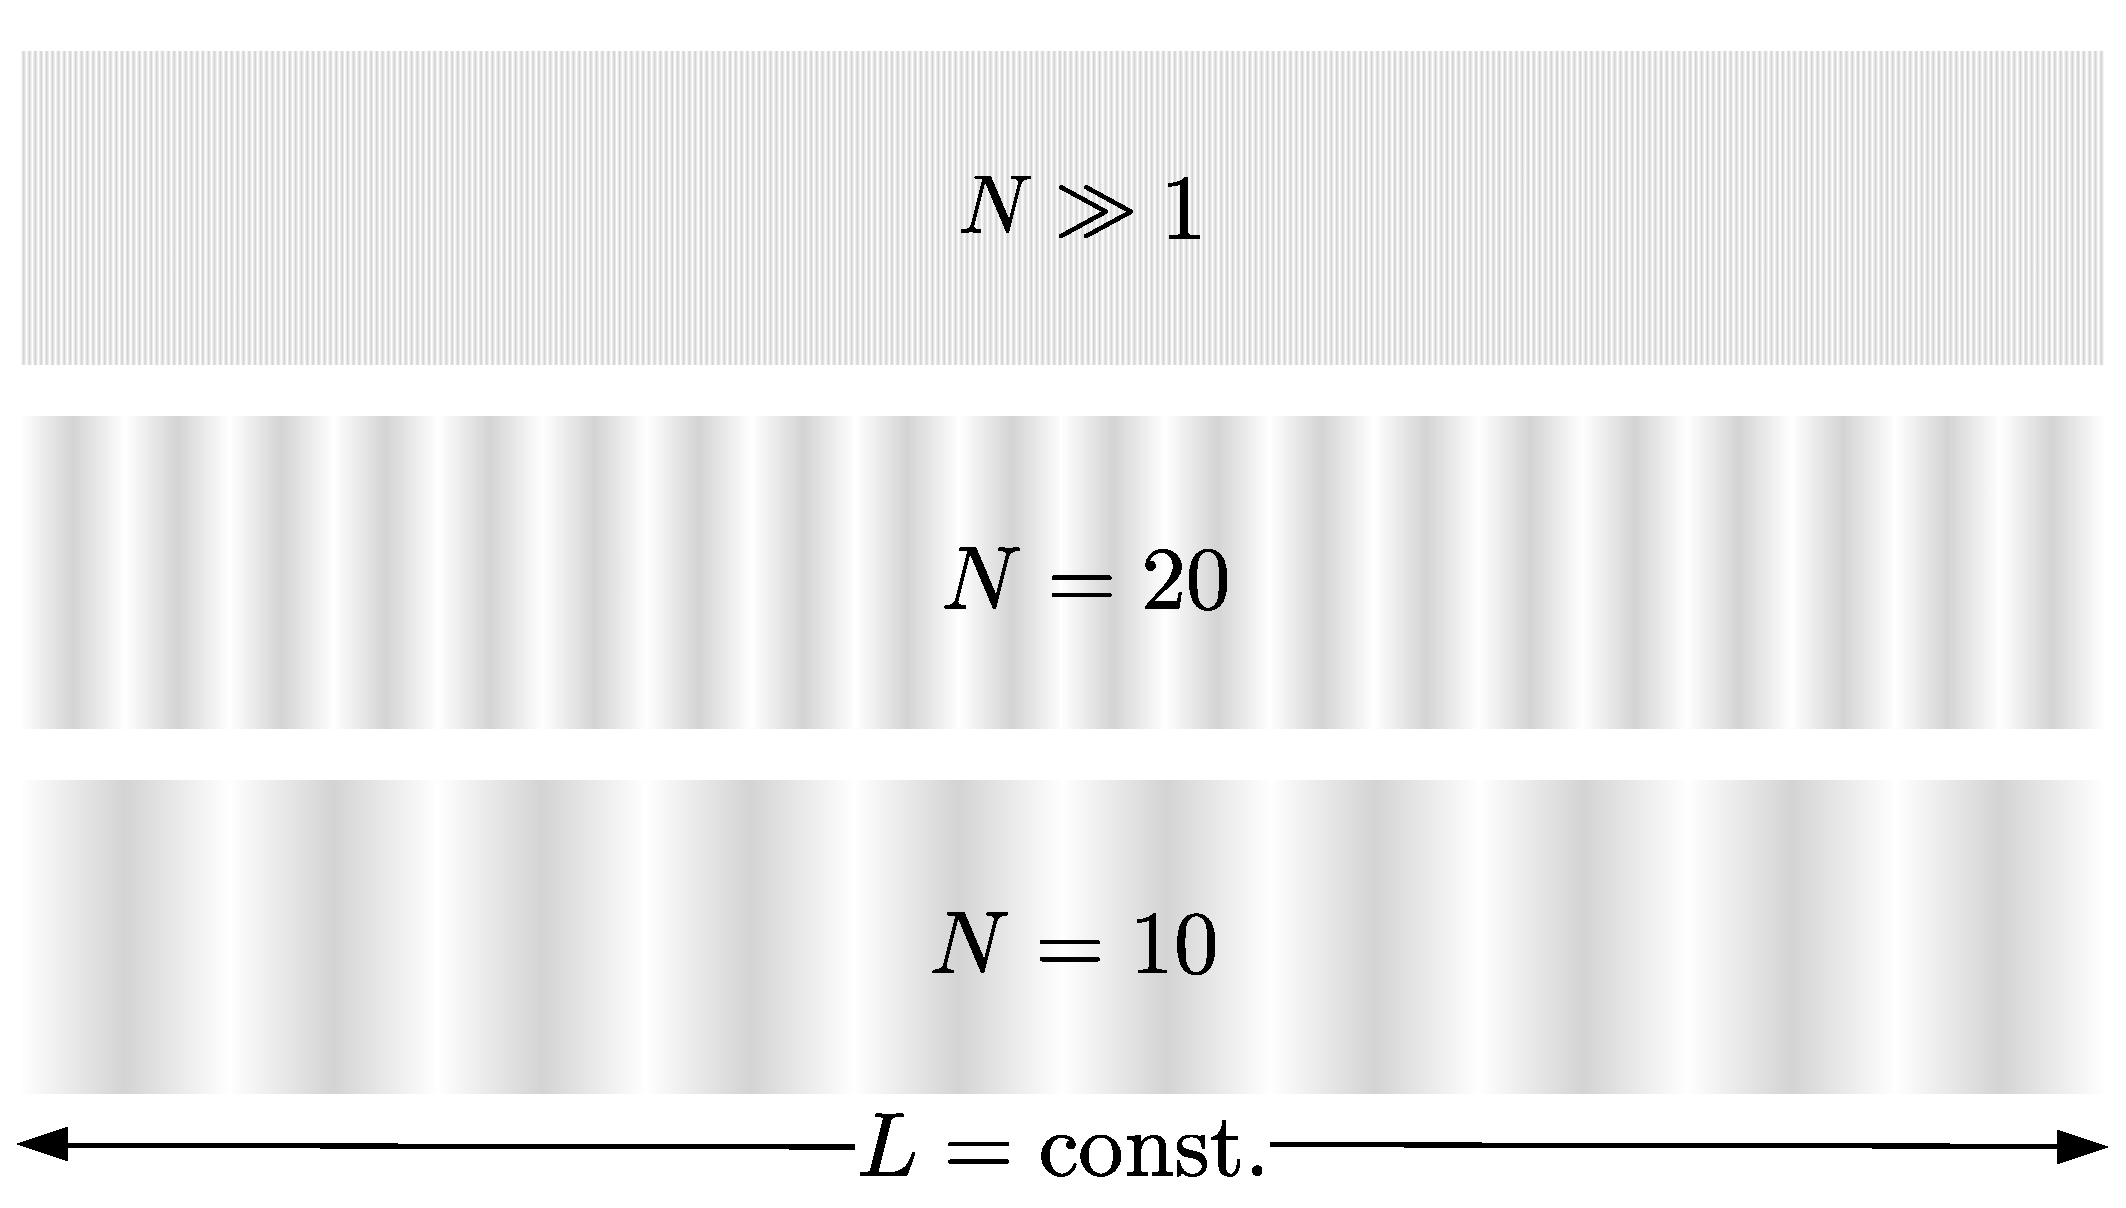
\includegraphics[width=0.6\linewidth]{Images/Chapter 2/Low N gratings.pdf}
    
    \caption{Illustrations of gratings with equal length but different layer numbers $N$, each providing near identical reflection zero locations $\wB \pm n\wz, \; n \in \mathbb{N}$.}
    
    \label{fig:Low_N_gratings}
\end{figure}
%
We therefore can calculate the required $\dt$ for a desired $\wz$ and $N$ through \eqref{eq:wz_approx}. The equivalence between different grating numbers is demonstrated in Figure~\ref{fig:discretised_EGM_accuracy}, where grating numbers $N \in [10, 22440]$ are used with near identical agreement. We therefore may select a layer number $N$ that is low enough to be amenable to standard numerical analyses such as continuation without encountering significant computational difficulties.
%
\begin{figure}[!t]
    \centering
    
    \begin{overpic}[width=0.75\linewidth]{Images/Chapter 2/discretised_EGM_accuracy.pdf}
        \put(4,78){(a)}
        \put(4,40){(b)}
    \end{overpic}
    
    \caption{Equivalence in EGM structure between different grating numbers $N \in [10, 22440]$ by keeping $N\dt$ constant.}
    
    \label{fig:discretised_EGM_accuracy}
\end{figure}
%
The key difference between using a low grating number is in the number of side lobes that are correctly modelled. Figure~\ref{fig:discretised_EGM_wide_view} plots the EGM solution curves over $\w_s \in [-20\wz, 20\wz]$ for $N = 10$ and $N = 22440$ while keeping $N\dt$ constant. It can be seen that when $N=10$, a main reflection lob appears after every $10\wz$, meaning that five side lobes are obtained before the model becomes completely non-physical. In contrast, the side lobes continue for the true grating number for 1550 nm light. Overall, a balance must be made between choosing an $N$ that is low enough so that the system is still amenable to analysis through integration and continuation, while not introducing non-physical features to the EGM structure over the parameter region being studied. To this end, we illustrate two undesirable situations that can occur for an insufficiently large $N$ in Figure~\ref{fig:discretised_EGM_minimumN}, which plots EGM solutions for $N=10$ for varying detuning $\wB$. The valid solution regions, corresponding to a frequency range of $\pm 5 \wz$, are plotted with opaque lines while the entire frequency region is plotted with semi transparent lines. The first case demonstrated in the left column illustrates how if the detuning $\wB$ becomes large enough, the valid portion can be completely detuned away from $\w_s=0$ as shown in the progression from (a1) to (b1). As the amplitude of side lobes will begin to increase again past this point as shown in (c1) (where they should continue to diminish) one could find larger EGM regions than is physically correct. This can be avoided by ensuring that over the parameter region being studied, $N$ is larger than $2{\w}_{B, \max}/{\w}_{z,\min}$. The second and perhaps more problematic case shown on the right column, occurs when repeated side lobes intersect the line $f(\w_s) = \w_s$. and the repeated main reflection lobes over the entire parameter region of interest. The first repetitions of the main lobe occur at $\w_s = \pm N \wz + \wB$, while each main lobe has a maximum at $\pm \eta \sqrt{1+\a^2}$. The line $f(\w_s)$ can therefore hit the first repeated main lobes at $\w_s = \pm \eta \sqrt{1+\a^2}$. For $\wB=0$ as shown in (a2), only valid regions of the EGM envelope intersect the line $f(\w_s)$, but as $\wB$ increases, the first repeated main lobe begins to intersect $f(\w_s)$ at $\w_s = \pm \eta \sqrt{1+\a^2}$ as shown in (b2), introducing invalid EGM components to the solution structure as $\wB$ is increased as shown in (c2). Note that detuning is not the only mechanism for which this can occur, for example, increasing the feedback rate $\eta$ in (b1) would increase the amplitude of the solution envelope and quickly cause intersections between the repeated main lobes and $f(\w_s)$. To guarantee these non-physical features are not introduced into the EGM structure, we therefore require the first repeated peaks to never be within $\w_s = \pm \eta \sqrt{1+\a^2}$, which can be ensured through
%
\begin{equation*}
    N \wz + |\wB| > \w_s = \eta \sqrt{1+\a^2}
\end{equation*}
%
Combining these two conditions, a lower bound on the grating number $N$ for a particular parameter region can then be prescribed as
%
\begin{equation}
    \label{eq:Nmin}
    N_\text{min} = \max \left\{ \left\lceil \frac{2|\wB|_{max}}{\w_{z,\min}} \right\rceil , \;\left\lceil \frac{|\wB|_{\max} + \eta_{\max} \sqrt{1+\a_{\max}^2}}{\w_{z,\min}} \right\rceil \right\}
\end{equation}
%
\begin{figure}[!t]
    \centering
    
    \includegraphics[width=0.75\linewidth]{Images/Chapter 2/discretised_EGM_wideview.pdf}
    
    \caption{EGM solutions over a wide frequency range $\w_s \in [-20\wz, 20\wz]$ for two different grating numbers $N = 10$ and $N = 22440$ while keeping $N\dt$ constant.}
    
    \label{fig:discretised_EGM_wide_view}
\end{figure}
%
\begin{figure}[!t]
    \centering
    
    \includegraphics[width=0.94\linewidth]{Images/Chapter 2/discretised_EGM_minimumN.pdf}
    
    \caption{EGM solutions for varying detuning $\wB$ with $\wz=0.1$ (left) and $\wz=0.02$ (right) and $N=10$ in both cases. Valid region solution regions are plotted with opaque lines while the entire frequency region is plotted with semi transparent lines.}
    
    \label{fig:discretised_EGM_minimumN}
\end{figure}
%
While a low reflectivity $R$ does provide the desired transmission zeros, the relative errors in both total reflectivity $R_\text{error}$ and delay $\tau_\text{error}$ are larger compared to larger total reflectivities. This is demonstrated in Figure~\ref{fig:NR_Selection}, which visualises the combined relative errors $R_\text{error}$ and $\tau_\text{error}$ using the Euclidean metric $\| R_\text{error}, \tau_\text{error} \|_{_2} = \sqrt{R_\text{error}^2 + \tau_\text{error}^2}$. For the choice $N=10$, a total reflectivity $R_\text{approx} = 0.75$ would provide a lower combined error of 4\% as shown in (a) compared to the $R_\text{approx} = 0.1$ which has a combined error of 19\%. As the ability to effectively describe and analyse transmission zeros of FBGs is of great interest, this increase in combined error, which is still relatively low from a modelling perspective, is a an acceptable trade-off.
\begin{figure}
    \centering
    
    \begin{overpic}[width=0.8\linewidth]{Images/Chapter 2/NR Selection large R.pdf}
        \put(0,34){(a)}
    \end{overpic}\\[0.5em]
    \begin{overpic}[width=0.8\linewidth]{Images/Chapter 2/NR Selection low R.pdf}
        \put(0,40){(b)}
    \end{overpic}
    
    \caption{figure}{Combined relative errors of FBG total reflectivity $R_\text{error}$ and delay $\tau_\text{error}$ as a function of the grating number $N$ and normalised refractive index variation $\dn$. Level sets of constant total reflectivity $R_\text{approx}$ are overlayed in white. In (a), the square marker at $(N,\dn) = (10, 0.07)$, corresponding to an $R_\text{approx} = 0.75$ has a combined error of 4\% while in (b), the marker at $(N,\dn) = (10, 0.0055)$, corresponding to an $R_\text{approx} = 0.1$ has a combined error of 19\%.}
    
    \label{fig:NR_Selection}
\end{figure}
%
\par
%
Note then, that the final grating parameter $\dt$, which determines the grating length $L$, controls the grating bandwidth. The effective feedback rate is defined as $\eta_{eff} \equiv \eta R$. We can now compare the two derived models describing FBG distributed feedback. The first of which derived directly from the FBG reflection spectrum $\rho(\w)$ using Lorentzian distributions, and the present model, approximating the FBG impulse response $\tilde{\rho}(t)$. We compare EGM solutions of both models using identical parameters in Figure~\ref{fig:discretised_3Lorentzian_EGM_comparison} where results obtained by the discretised reflections model are plotted with solid lines and round markers, while results obtained by the Lorentzian model are plotted with dashed lines and square markers. Remarkable agreement between these models can be seen, in spite of their independent derivations. The nulls of the envelopes of $f(\w_s)$ in both cases agree precisely, while their values at $\w_s=0$ only show slight disagreement, due to the error in total reflectivity in the discretised reflection model for $R=0.01$. Further, both models predict 11 EGMs with excellent agreement in their locations. As the Lorentzian model has a more physically concrete derivation, this gives strong evidence as to the physical relevance of the discretised reflection model, while having the added benefit of modelling side lobes of the reflection spectrum. 
%
\begin{figure}[!t]
    \centering
    
    \begin{overpic}[width=0.75\linewidth]{Images/Chapter 2/discretised_threeLorentzian_EGM_comparison.pdf}
        \put(4,78){(a)}
        \put(4,40){(b)}
    \end{overpic}
    
    \caption{EGM solutions of the Lorentzian and discretised reflection model using identical parameter values. Results obtained by the discretised reflections model are plotted with solid lines and round markers, while results obtained by the Lorentzian model are plotted with dashed lines and square markers.}
    \label{fig:discretised_3Lorentzian_EGM_comparison}
\end{figure}
%
\par
%
\section{Comparison to previously studied FBG feedback models}
\label{sec:model_comparison}
%
Given the excellent agreement in ECMs confined to the main lobe between the three Lorentzian model and the discretised reflection model, we now compare agreement in solution structure and system dynamics between the discretised reflection model and the various approaches to modelling the feedback term $F(t)$ within the LK equations in the literature. This section demonstrates the excellent agreement this discretised model demonstrates with significantly less computational effort, while portraying several analysis techniques available to this system that is not possible with previously studied forms of FBG feedback. 
%
%
\subsection{EGM Accuracy}
\label{subsec:naumenko}
A considerably more complex system presented by Naumenko \textit{et al.} in \cite{naumenko2003characteristics} considers the feedback term $F(t)$ in the form of \eqref{eq:multiple_EC} that is, as the inverse Fourier transform of the product of the time delayed electric field in the spectral domain $\mathcal{F}[E(t-\tau)](\w)$ and the grating reflection spectrum $\rho(\w)$. The model additionally considers nonlinear gain and frequency chirp due to thermal effects when the injection current is changed. Ignoring these additional effects, and making suitable approximations, the system simplifies to the derived discretised reflection system as shown in Appendix~\ref{sec:multiple_EC_nondim} with parameter values $(\a, P, T, \tau, C_p) = (4, 0.5, 123, 512, 0)$, and varying grating parameters $\eta$, $\wB$, and $\wz$.
%
\par
%
EGMs were calculated with the help of Green functions through an involved mathematical procedure, as opposed to deriving closed form analytical equations. As discussed in the introduction, they identified `satellite' EGMs, separated from the central EGM envelope by the zeros of the main lobe by varying both grating bandwidth $\wz$ and detuning $\wB$.
%
\begin{figure}[!t]
    \centering

    \begin{minipage}[t]{0.43\textwidth}
        \vspace*{0pt}
        \begin{overpic}[width=\linewidth]{Images/Chapter 2/rB_003_annotated.pdf}
            \put(4,96){(a1)}
            \put(4,45){(b1)}
        \end{overpic}
    \end{minipage}
    \hspace{2em}
    \begin{minipage}[t]{0.4\textwidth}
        \vspace*{0em}
        \begin{overpic}[width=\linewidth]{Images/Chapter 2/Naumenko_rB003.pdf}
            \put(0,68){(a2)}
        \end{overpic}
        \vskip 1.0em
        \hspace{0.0em}
        \begin{overpic}[width=0.97\linewidth]{Images/Chapter 2/Naumenko_EGM_rB003.pdf}
            \put(-3,77){(b2)}
        \end{overpic}
    \end{minipage}
   
    \caption{A comparison between EGMs in the multiple reflection (left) and discretised FBG (right) models in the frequency-intensity domain for varying grating bandwidth and zero detuning. The curves in panels (a1) and (a2) illustrate the FBG frequency responses. A constant reflectivity of $R=0.0316$ yields a nondimensionalised effective feedback rate $\eta=0.085$ while Bragg grating reflection zeros at 1/3, 4/3, and 20/3 GHz yield nondimensionalised reflection zero locations $\wz=0.016\pi, \; 0.064\pi, \; 0.32\pi$. The EGMs in panels (b1) and (b2) corresponding to these respective bandwidths are plotted with circles $(\circ)$, diamonds $(\diamond)$ and squares $(\square)$, while the MGM in each case is plotted indicated by a $\times$.}
    
    \label{fig:Naumenko_rB003}
\end{figure}
%
\begin{figure}[!t]
    \centering
    
    \begin{minipage}[t]{0.45\textwidth}
        \vspace{0pt}
        \begin{overpic}[width=\linewidth]{Images/Chapter 2/rB_02_annotated.pdf}
            \put(4,94){(a1)}
            \put(4,46){(b1)}
        \end{overpic}
    \end{minipage}%
    \hspace{1em}
    \begin{minipage}[t]{0.4\textwidth}
        \vspace{0.5em}
        \begin{overpic}[width=\linewidth]{Images/Chapter 2/Naumenko_rB02.pdf}
            \put(0,69){(a2)}
        \end{overpic}
        \vskip 0.5em
        \hspace{0.2em}        
        \begin{overpic}[width=0.96\linewidth]{Images/Chapter 2/Naumenko_EGM_rB02.pdf}
            \put(-3,79){(b2)}
        \end{overpic}
    \end{minipage}

    \caption{A comparison between EGMs in the multiple reflection (left) and discretised FBG (right) models in the frequency-intensity domain for a detuned FBG. A reflectivity of $R=0.224$ yields a nondimensionalised effective feedback rate $\eta=0.600$ while a Bragg grating reflection zero at 10/3 GHz yields nondimensionalised reflection zero location $\wz=0.16\pi$. Finally, a detuning of 8 GHz corresponds to $\wB=0.384\pi$.}
    
    \label{fig:Naumenko_rB02}
\end{figure}
%
Figures~\ref{fig:Naumenko_rB003} and \ref{fig:Naumenko_rB02} compare results obtained by both the multiple EC reflection FBG feedback and discretised FBG models for varying grating reflectivity, bandwidth and detuning. In order to to obtain valid EGM solutions, for both parameter sets, $N=10 > N_\text{min}=7$ was used. Solutions are projected in the frequency-intensity plane where $I = |E|^2$, in contrast to the usual projection in the inversion-frequency plane, causing an inversion of the cavity modes about the frequency axis. The photon lifetime $\tau_p=24\,\text{ps}$ was used to convert grating bandwidths in Hz to their nondimensionalised $\wz$ form. Clearly, excellent agreement in the mode structure is achieved, in particular for the low feedback rate case. Firstly, considering no detuning, low feedback and varying bandwidths as is the case in Figure~\ref{fig:Naumenko_rB003}, for a wide bandwidth of the Bragg reflector (in this case, a main lobe width of 40/3 GHz or $2\wz=0.64\pi$ in nondimensionalised form), EGMs lie on a closed curve, resembling a COF ECM structure, as expected. The MGM (mode with highest power) is located for near the edge of the left side of the closed curve, indicated by an '$\times$' in the figure. As the FBG bandwidth is decreased, the number of EGMs decreases, and the EGM solution curve and MGM narrows as they are confined to within the bandwidth of the main lobe, in agreement with results obtained from Sections~\ref{sec:EGM_Lorentzian} and \ref{sec:EGM_discretised} and with results obtained for a single Lorentzian filter \cite{yousefi1999dynamical}. Further narrowing the filter bandwidth introduces satellite EGMs, indicated with triangles, due to the side lobes of the FBG reflection spectrum. It is noted that this effect does not occur in the single Lorentzian filter for zero detuning. At this point, the MGM as nearly at the Bragg frequency, in agreement with physical intuition. Increasing the feedback rate considerably, and detuning the FBG from the laser's free-running frequency, as shown in Figure~\ref{fig:Naumenko_rB02}, also detune the EGM modes, and split the modes into three disjoint curves, corresponding to the main lobe and two side lobes nearest to the laser's free-running frequency. This splitting of solution curves was similarly observed for the single Lorentzian filter \cite{yousefi1999dynamical}, but at most two disjoint curves can be formed \cite{green2006mode}, while in this case already three distinct solution curves are present. Significant distortion in the EGM structure along the intensity axis can be seen for the discretised reflection case compared to the Multiple EC reflection model, which can be attributed to the lack of a gain suppression factor in this model in this simplified model. In any case, excellent agreement in the locations of the EGM components, MGM, and number of EGM solutions demonstrates the ability of the discretised reflections model to capture the solution structure of FBG feedback.
%
\par
%
% \begin{figure}[!t]
%     \centering
    
%     \begin{overpic}[width=0.8\linewidth]{Images/Chapter 2/Li_P1_local_minima.png}
%         \put(4,78){(a1)}
%         \put(54,78){(a2)}
%     \end{overpic}
%     \vskip 0.5cm
%     \hspace{-0.2cm}
%     \begin{overpic}[height=0.3\linewidth]{Images/Chapter 2/Li_chaos_FBG_extrema_001eta02.pdf}
%         % \put(4,78){(b1)}
%     \end{overpic}   
%     \hspace{0.0cm}
%     \begin{overpic}[height=0.3\linewidth]{Images/Chapter 2/Li_chaos_mirror_extrema_001eta02.pdf}
%         % \put(4,78){(b2)}
%     \end{overpic}    
%     \caption{}
%     \label{fig:P1_comparison}
% \end{figure}
%
%
\subsection{Stability Fluctuations}
\label{subsec:lichaos_skenderas}
%
%
It is important to note that while the locations of zeros in the discretised model are uniform, is only the case for FBGs which have relatively low reflectivities, see Figure~\ref{fig:uniform_spectra_varykL}. For this, re
%

\begin{figure}[p]
    \centering
    
    \begin{minipage}[t]{0.44\textwidth}
        \begin{overpic}[width=\linewidth]{Images/Chapter 2/Li_chaos_heatmap.png}
            \put(-2,85){(a)}
        \end{overpic}
    \end{minipage}%
    \hspace{0.5em}
    \begin{minipage}[t]{0.46\textwidth}
        \raisebox{-1em}{%
            \begin{overpic}[width=\linewidth]{Images/Chapter 2/discretised_Lichoatic_wBeta_comparison.pdf}
                \put(-2,85){(b)}
            \end{overpic}
        }
    \end{minipage}
    \\
    \begin{minipage}[t]{0.9\textwidth}
        \vspace{0.2em}
        \begin{overpic}[width=\linewidth]{Images/Chapter 2/discretised_Lichoatic_wBeta_xy_forwardbackward_comparison_lyapunov.pdf}
            \put(-2,68){(c)}
        \end{overpic}
    \end{minipage}

    \caption{Comparison between two parameter dynamical mappings of output intensity for a convolved FBG feedback form of $F(t)$ \cite{li2012distributed,li2015chaotic,li2020stable} (a) and the discretised FBG feedback form of $F(t)$ in the parameter space of feedback strength ($\xi_f$ in (a) and equivalent $\eta$ in (b)) and grating detuning frequency ($\Delta f$). In (a), the laser output intensity is stable (white), period-one oscillatory (red), quasi-periodic pulsating (gray), period-doubled oscillatory (yellow), and chaotic (black). In (b), the laser output is in steady-state (white), period-one oscillatory (red), period-two (yellow), and period 3 to very large period in a gradient from grey to black. In (c) parameter sweeps are performed in all four directions, with Hopf bifurcations of steady state EGMs overlayed}
    
    \label{fig:Li_chaos}
\end{figure}
%
\par
%
Finally, we compare our model to the most recent work on semiconductor lasers under FBG feedback by \Skenderas \textit{ et al.} \cite{skenderas2021feedback,skenderas2024impact}. In contrast to the previous two models, where nondimensionalisations and approximations were required before direct comparisons could be made, the form of the equations analysed mirror the equations presented in this work, using parameter values $(\a, P, T, \tau) = (3, 1, 1000, 1000)$, except for the use of a convolution feedback term $F(t)$ of the form \eqref{eq:convolution}. The results presented by \Skenderas \textit{ et al.} therefore serve as the most suitable basis for comparisons in the accuracy of the derived discretised model. Given the complexity of analysing the LK equations under FBG feedback using a convolution term, the results presented, like those previously studied, are obtained solely through analysis of time series obtained through numerical integration. The main focus of their analysis is in characterising the interplay between the lasers relaxation oscillations (ROs) and the FBG reflection zeros as a function of feedback rate $\eta$ and grating bandwidth $\wz$ for varying feedback phase $C_p$ and grating detuning $\omega_B$. 

ROs are the most typical type of oscillation that one would expect in semiconductor lasers. They are damped intensity fluctuations that occur when the laser transitions between steady states, typically after a sudden change in injection current, and arise from the dynamic interplay between photon density and carrier density in the laser cavity. When the carrier population is perturbed, it overshoots the steady-state value, causing oscillations in output power at a characteristic frequency known as the relaxation oscillation frequency $\w_\text{RO}=\sqrt{2P/T}$, which form the dominant side lobes either side of the centre frequency in the Fourier spectrum of a semiconductor laser. Exciting the ROs of a laser can lead to a more unstable laser, and therefore one would expect that lower amount of feedback would cause the laser to transition from steady output to oscillatory and then more unstable outputs. 

The strategy employed by the authors to observe They do this by tracking the Hopf bifurcation of the steady state of the laser in the $(L_\text{FBG},\eta)$-plane, where the grating length $L_\text{FBG}$ can be used to control the grating bandwidth $\wz$ as discussed in \ref{sec:EGM_discretised}. As discussed in \ref{sec:FBG}, varying the grating length also changes the grating reflectivity, therefore, when using this model, grating parameters must be simultaneously varied to solely vary its bandwidth. This is not an issue with the discretised reflections model as bandwidth $\wz$ and thus length $L_\text{FBG}$ can be varied independent of reflectivity using \ref{eq:wz_approx}
%
\begin{equation}
    L [\text{m}] \approx \frac{\pi c \tau_p}{\wz \neff} 
\end{equation}
%
where $\tau_p$ is the photon lifetime used to rescale time in this form of the LK equations as discussed in Section~\ref{sec:EGM_discretised}.
%
\par

%
\begin{figure}[!t]
    \centering   
    \includegraphics[width=0.75\linewidth]{Images/Chapter 2/discretised_Skenderas_wzeta_Cpcomparison_N20.pdf}    
    \caption{The evolution of Hopf bifurcation tracking the stability fluctuations as a function of $L_\text{FBG}$ at zero detuning for different values of the feedback offset phase $C_p$ equal to $0$ (blue), $\pi /4$ (yellow), $\pi/2$ (violet), $2\pi/3$ (green), $\pi$ (cyan), $3\pi/2$ (maroon), and $7\pi/4$ (orange).}
    \label{fig:Skenderas_Hopf_Cpvars}
\end{figure}
%
\begin{figure}[p]
    \centering
    
    \begin{minipage}[t]{0.45\textwidth}
        \begin{overpic}[width=\linewidth]{Images/Chapter 2/discretised_Skenderas_wBeta_image.pdf}
            \put(-5,80){(a)}
        \end{overpic}
    \end{minipage}%
    \hspace{0.5em}
    \begin{minipage}[t]{0.45\textwidth}
        \raisebox{0em}{%
            \begin{overpic}[width=\linewidth]{Images/Chapter 2/discretised_Skenderas_wBeta_comparison.pdf}
                \put(-5,80){(b)}
            \end{overpic}
        }
    \end{minipage}
    \\
    \begin{minipage}[t]{0.94\textwidth}
        \begin{overpic}[width=\linewidth]{Images/Chapter 2/discretised_Skenderas_wBeta_xy_forwardbackward_comparison.pdf}
            \put(-2,65){(c)}
        \end{overpic}
    \end{minipage}

    \caption{Comparison between two parameter dynamical mappings of output intensity for a convolved FBG feedback form of $F(t)$ \cite{li2012distributed,li2015chaotic,li2020stable} (a) and the discretised FBG feedback form of $F(t)$ in the parameter space of feedback strength ($\xi_f$ in (a) and equivalent $\eta$ in (b)) and grating detuning frequency ($\Delta f$). In (a), the laser output intensity is stable (white), period-one oscillatory (red), quasi-periodic pulsating (gray), period-doubled oscillatory (yellow), and chaotic (black). In (b), the laser output is in steady-state (white), period-one oscillatory (red), period-two (yellow), and period 3 to very large period in a gradient from grey to black. In (c) parameter sweeps are performed in all four directions, with Hopf bifurcations of steady state EGMs overlayed}
    
    \label{fig:Skenderas_wBeta}
\end{figure}
%

